\documentclass[12pt]{article}

\usepackage{graphicx}

\title{CS 372 Lab 5: Ethernet}
\author{Ian Kronquist}

\begin{document}
\maketitle

\begin{enumerate}
    \item Source: ac:bc:32:85:1c:ff
        \begin{figure}[!ht]
            \centering
            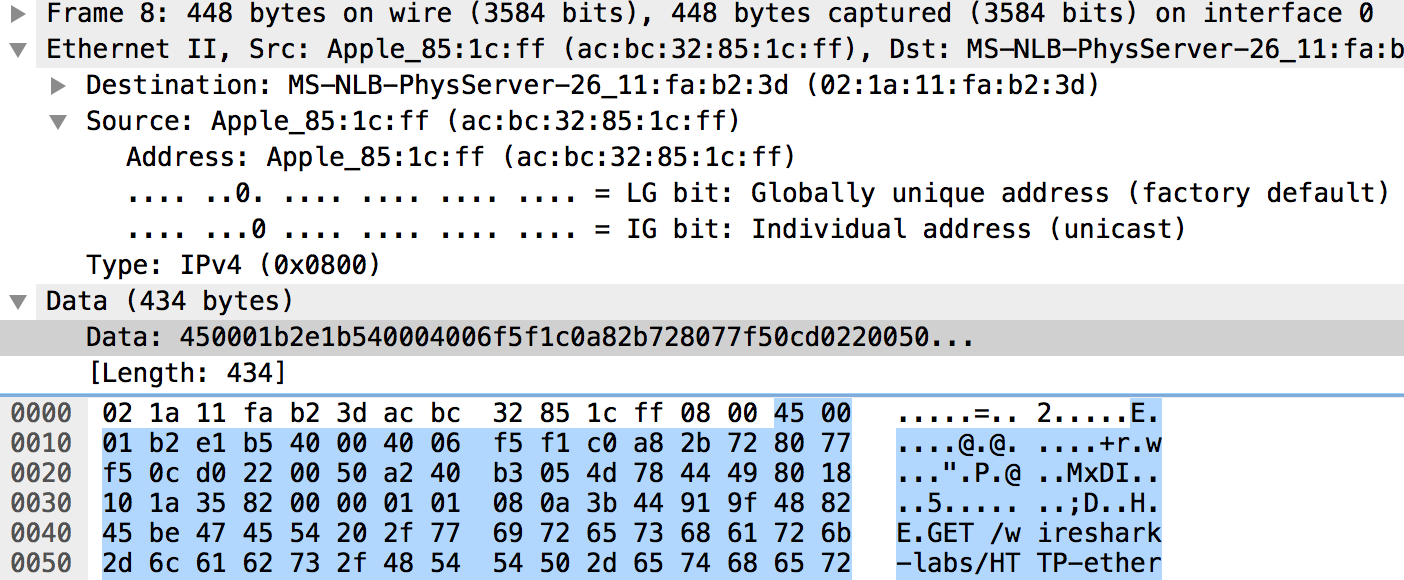
\includegraphics[scale=0.5]{./p1.eps}
            \caption{Ethernet frame}
        \end{figure}
    \item Destination: 02:1a:11:fa:b2:3d. This is the address of the router for
        my network.
    \item The frame type is 0x0800, which represents IPv4.
    \item It is 66 bytes from the very start of the Ethernet frame.
    \item The value of the source address is 02:1a:11:fa:b2:3d
    \item The destination address is my computer's, that is ac:bc:32:85:1c:ff.
    \item The frame type is still IPv4, with code 0x0800.
    \item The O in OK appears at byte 79.
    \item Running \texttt{arp -a} on OS X gives the following output.
        \begin{verbatim}
        ? (192.168.5.255) at (incomplete) on vmnet1 ifscope [ethernet]
        ? (192.168.43.1) at 2:1a:11:fa:b2:3d on en0 ifscope [ethernet]
        ? (192.168.43.255) at (incomplete) on en0 ifscope [ethernet]
        ? (192.168.145.255) at (incomplete) on vmnet8 ifscope [ethernet]
        ? (224.0.0.251) at 1:0:5e:0:0:fb on en0 ifscope permanent [ethernet]
        \end{verbatim}
        You can see that I have three network interfaces, vmnet1, vmnet8, (used
        for routing to and from local virtual machines) and en0 (for ethernet).
        All of these communicate over ethernet. Each entry has an IP address,
        and entries over the en0 interface all have Ethernet addresses
        associated with the IP addresses.
    \item Source: 00:d0:59:a9:3d:68
        Destination: ff:ff:ff:ff:ff:ff
    \item The ethernet frame type is 0x0806. This corresponds to the ARP
        protocol.
    \item 
        \begin{enumerate}
            \item The opcode begins at byte 20.
            \item The value of the opcode field is 1.
            \item The ARP request includes the local IP address of the sender.
            \item The ARP question occurs at byte 38.
        \end{enumerate}
    \item
        \begin{enumerate}
            \item The arp opcode begins at byte 20.
            \item The value of the opcode field is 2.
            \item The target address of the opcode is at byte 38.
        \end{enumerate}
    \item Source: 00:06:25:da:af:73
        Destination: 00:d0:59:a9:3d:68.
    \item There may have been a reply, but it wasn't picked up by the computer
        which made the original trace since it wasn't sent to that machine.

    \item We would get a duplicate arp table entry. The arp table entry would
        be registered as 'permanent' and would have to be removed twice to
        fully clean up both entries.
    \item According the manual entry for the ARP(8) protocol, routes are
        normally kept for 20 minutes after being validated.

\end{enumerate}

\end{document}
